% Copyright (C) 2013 Thomas L. Kula
% All Rights Reserved
%
% See the file LICENSE for license terms.
\documentclass[12pt]{article}
\usepackage{graphicx}
\usepackage{rotating}
\usepackage{fix-cm}
\usepackage{multirow}
\setlength{\paperwidth}{5.5in}
\setlength{\paperheight}{8.5in}
\setlength{\textheight}{7.45in}
\setlength{\topmargin}{-1.0in}
\setlength{\oddsidemargin}{-0.5in}
\setlength{\evensidemargin}{-0.5in}
\setlength{\textwidth}{4.0in}
\setlength{\parindent}{0in}
\setlength{\parskip}{3mm}
\usepackage[print]{booklet} \nofiles
\source{\magstep0}{5.5in}{8.5in}
\target{\magstep0}{11in}{8.5in}
\setpdftargetpages
\pagestyle{empty}
\begin{document}


\begin{center}
{\fontsize{36}{48}\selectfont \textsc{Haiku a Day }}
\end{center}

\vspace*{3.5cm}

{\fontsize{20}{40}\selectfont 

A twitch of the eye

Snow flying, but not for long

Winter's hand fading


}

\vspace*{5.0cm}
\begin{center}
{\large{Issue 91: January 2013}} \\[5mm]
{\fontsize{8}{8}\selectfont  \textsc{ St. Joshua Norton Press }} \\[1mm]
{\fontsize{6}{6}\selectfont Mathom House by the Cloisters \textbar The People's Republic of Ames }
\end{center}


\newpage

I like winter, I like cold weather. But I've had my blizzard. It's time for Spring.

--- Thomas

http://kula.tproa.net/had/ \\
kula@tproa.net

Download this and previous HADs at the website, so you can
print out your own (DIY, yeah!) or if you want me to send
you one, send me your address, and maybe a stamp if you
are feeling nice. Or send me something you've made ---
trades always appreciated, postcards are nice too.

\vfill

1 January 2013

By the East River \\
The city reminds me just \\
How lucky I am

2 January 2013

What's that sensation? \\
Upcoming feeling of doom --- \\
Just my alarm clock

3 January 2013

Similarity \\
Two containers look the same \\
The one I grab wrong

\newpage

4 January 2013

Sometimes things don't work \\
Key is to take the pieces \\
And make something else

5 January 2013

Time for a movie. \\
Which one do I want to see? \\
Then hours pass by.

6 January 2013

Don't know direction \\
Know the feel of the city \\
My feet get me there

7 January 2013

In my conviction \\
This thing works a certain way \\
In reality...

8 January 2013

The must on the grapes \\
A must when you're making wine? \\
Or must you remove?

9 January 2013

A simple mixture \\
Each brings a contribution \\
Yummy food forthwith

10 January 2013

First night Trevoring \\
Answering Trevor letters \\
After, there are chips

\newpage

11 January 2013

Beacons around me \\
Where there is pizza, there's hope \\
I buy some slices

12 January 2013

What is this acid \\
Never heard of it before \\
Sitting in my food

13 January 2013

Hanging from the wall \\
A lone spider thread --- not web \\
Dusting takes care of

14 January 2013

Too much junk in here \\
Some things are destined for scrap \\
Or a flamethrower

15 January 2013

Evening of Awesome \\
People who are amazing \\
Fill Carnegie Hall

16 January 2013

An alternate dish \\
When the main ingredient \\
Isn't at the store

17 January 2013

Nerding out over \\
Marshall Kirk McKusick's talk \\
BSD book signed

\newpage

18 January 2013

An act in three parts \\
Concerto for bubbling pipes \\
Bubble, squeak and hiss

19 January 2013

Read about the brain \\
Making my brain think of brains \\
A headache ensues

20 January 2013

We start with a plan \\
And minutes in that goes out \\
Winging it from here

21 January 2013

Tamale making \\
Is a very refined craft \\
I need more practice

22 January 2013

An idea flashes \\
Last minute horchata made \\
Why'd I wait so long?

23 January 2013

Feeling off today \\
But a walk as always helps \\
It's cheap therapy

24 January 2013
 
Every minute last \\
Something always must be done \\
The list keeps going

\newpage

25 January 2013

The plane lands, a bump: \\
Iowa! Pigs and corn reign! \\
All sits before me

26 January 2013

Pardon me today \\
I have a niece to spoil \\
No one else matters

27 January 2013

A sink of dishes \\
An hour of happy swish \\
House meditation

28 January 2013

Knives flashing, food flies \\
A hot griddle a palate \\
An artist cooking

29 January 2013

The wind swiftly moves \\
Scouring the ground, freshly \\
Now covered in snow

30 January 2013

Leaving the bubble \\
Going out for some shopping \\
Good to be back home

31 January 2013

The closet, my coat \\
The handle broken, I'm stuck \\
Not going outside


\newpage

\begin{center}
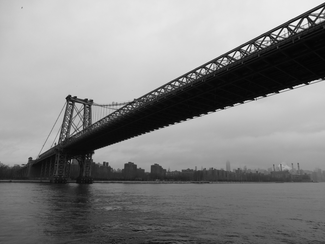
\includegraphics[width=325pt]{bridge.png}
The Williamsburg Bridge \\
12 January 2013 \\
{\tt kula.tproa.net/photos/2013/20130112-touring-nyc }
\end{center}

\newpage

\thispagestyle{empty}
\vspace*{12cm}
\begin{sideways}
\Large{St. Joshua Norton Press}
\end{sideways}
\begin{sideways}
\Large{PO Box 250138}
\end{sideways}
\begin{sideways}
\Large{New York NY 10025}
\end{sideways}


\end{document}


